% Extended version: full formulation, implementation detail, all results and limitations.
% Compile: pdflatex paper_extended; bibtex paper_extended; pdflatex paper_extended; pdflatex paper_extended
\documentclass[11pt]{article}
\usepackage[margin=1in]{geometry}
\usepackage[T1]{fontenc}
\usepackage{times}
\usepackage{amsmath,amssymb,bm}
\usepackage{graphicx}
\usepackage{booktabs}
\usepackage{algorithm}
\usepackage{algpseudocode}
\usepackage[numbers,sort&compress]{natbib}
\usepackage{url}
\newif\ifextended\extendedtrue
\setlength{\emergencystretch}{3em}
\usepackage[hidelinks]{hyperref}
\usepackage{caption}
\captionsetup{font=small,labelfont=bf}
\renewcommand{\thesection}{\Roman{section}}
\renewcommand{\thesubsection}{\thesection.\Alph{subsection}}
\hypersetup{pdftitle={Soft Temporal Kernels for Graph Retrieval in Time-Sensitive Financial QA (extended version)}, pdfauthor={Shashvath M}}

\title{Soft Temporal Kernels for Graph Retrieval in Time-Sensitive Financial Question Answering: A Pre-registered Evaluation\\[4pt] \large Extended version}
\author{Shashvath M \quad and \quad Ramraj T\\[2pt]
\small Department of Computer Science and Engineering, Amrita School of Computing\\
\small Amrita Vishwa Vidyapeetham, Coimbatore, India}
\date{November 2026}

\begin{document}
\maketitle

\begin{abstract}
\noindent Temporal graph retrieval-augmented generation answers time-sensitive questions by keeping only facts whose timestamp lies inside the period a question asks about. The timestamps are written by a language model while the graph is built, so the 0/1 rule can discard useful evidence: in our graph, 9.9\% of stored facts carry a timestamp that is not even a valid calendar date. We replace the rule with a soft temporal kernel $\kappa = \exp(-\lambda d)$, where $d$ is the distance between a fact's timestamp and the asked period in a year--quarter--month--day tree, so that the original rule is the limit $\lambda \to \infty$. The kernel enters seed selection, the personalized PageRank walk and evidence scoring. We compare it with a question-independent decay and with time-partitioned hybrid keyword and dense seeding, and test it under controlled timestamp noise. All settings were fixed on a development set and the comparisons were pre-registered. On 152 test questions from six companies of the ECT-QA earnings-call benchmark, the kernel did not beat the verified baseline (Correct 0.603 vs 0.599; $\Delta = +0.004$, 95\% CI $[-0.049, 0.059]$). It changes the evidence for 110 of 116 answerable questions, helping multi-period questions and hurting single-period, multi-company ones. With 30\% of timestamps shifted it scored 0.627 vs 0.566, a trend that does not survive correction for multiple tests. This extended version adds the retrieval algorithm, the noise protocol in detail, the implementation and tests, all development and secondary results, a per-question breakdown, a case study and a discussion of threats to validity.

\medskip\noindent\textbf{Keywords:} retrieval-augmented generation; temporal knowledge graph; time-sensitive question answering; financial question answering; robustness
\end{abstract}

\section{Introduction}
Analysts and investors routinely ask questions such as ``What was Home Depot's revenue in the third quarter of 2022?'' or ``Which of these companies had the highest operating margin in 2021?''. Language models answer such questions poorly from memory, and retrieval-augmented generation (RAG) \cite{lewis2020rag} is the usual remedy: retrieve passages first, then answer from them. Earnings calls make the retrieval step unusually hard. Every quarter repeats the same phrasing with different numbers, so a passage from the wrong quarter looks almost identical to the right one, and an answer built on it is fluent and wrong.

Graph-based RAG organises a corpus as a knowledge graph and retrieves connected facts \cite{edge2024graphrag,guo2024lightrag,gutierrez2024hipporag}. TG-RAG \cite{han2025tgrag} adds time: each relation carries a timestamp, timestamps form a year--quarter--month--day hierarchy, and only relations dated inside the period named in the question may start the retrieval. On its earnings-call benchmark, ECT-QA, this filter is one of the method's main strengths.

The filter is all-or-nothing, however, and it filters on timestamps that a language model wrote while building the graph. In the graph we built, 832 of 8,408 stored facts (9.9\%) carry a timestamp that does not even follow a valid calendar form (``2023 QQ3'', ``Q1 2023'', ``LAST YEAR''). Correct timestamps can also be the wrong granularity: a full-year fact is excluded from a question about one of that year's quarters, and a neighbouring-quarter fact is excluded even when nothing from the exact quarter exists. In one of our development questions, none of the 60 most similar candidates carried the asked quarter, so the filter kept nothing and the model invented three figures.

This paper asks whether softening the filter helps. Our contributions are:
\begin{itemize}
  \item \textbf{A soft temporal kernel} $\kappa(\tau) = \max_{t \in T_q} \exp(-\lambda\, d_H(\tau, t))$ over a calendar tree, with one parameter, which equals the hard filter as $\lambda \to \infty$ (confirmed empirically).
  \item \textbf{Kernel-weighted retrieval}: the kernel is used in seed selection, in the personalized PageRank walk and in evidence scoring, and compared with a question-independent decay in the style of DyG-RAG \cite{sun2025dygrag} and with time-partitioned hybrid BM25 and dense seeding.
  \item \textbf{A timestamp-noise protocol} that shifts a controlled share of stored timestamps deterministically, so that every method sees identical noise.
  \item \textbf{A pre-registered evaluation}: the baseline is re-implemented and verified against the released code, all settings are fixed on a development set, and the test comparisons are written down before the single test run.
\end{itemize}
The main result is negative. On 152 held-out questions the soft kernel ties with the reproduced baseline (0.603 against 0.599 Correct). A per-question analysis shows why: the kernel changes the evidence for almost every question, helping multi-period questions and hurting single-period, multi-company ones. When stored timestamps are noisy, the hard filter degrades and the soft kernel does not; the gap at 30\% noise is significant on its own but not after correcting for multiple tests.

\section{Related Work}
\textbf{Retrieval-augmented generation.} RAG \cite{lewis2020rag} conditions a generator on passages retrieved by dense similarity. Passages are retrieved independently, which struggles when evidence is spread over documents or when many passages differ only in their period.

\textbf{Graph-based retrieval.} GraphRAG \cite{edge2024graphrag} extracts an entity graph and summarises communities of entities for corpus-level questions. LightRAG \cite{guo2024lightrag} pairs graph indexing with entity-level and theme-level retrieval. HippoRAG \cite{gutierrez2024hipporag} runs personalized PageRank (PPR) \cite{page1999pagerank,haveliwala2002topic} from the entities in a question to collect multi-hop evidence in one step. None of these models time.

\textbf{Temporal retrieval.} TG-RAG \cite{han2025tgrag} timestamps relations, organises the timestamps hierarchically, and restricts PPR seeding and evidence scoring to the asked periods; it also released ECT-QA. DyG-RAG \cite{sun2025dygrag} links events with weights that decay with their time difference. Those weights are fixed at build time and ignore the question; our ablation B1QI isolates exactly this difference. Time-sensitive QA benchmarks such as TimeQA \cite{chen2021timeqa} show that models fail when the answer changes with the time expression.

\textbf{Hybrid retrieval and evaluation.} BM25 \cite{robertson2009bm25} captures exact tokens (tickers, ``EPS'', ``Q3'') that dense vectors blur, and Reciprocal Rank Fusion (RRF) \cite{cormack2009rrf} merges rankings without score calibration. We follow TG-RAG's element-level LLM-judge protocol, which agrees reasonably with human raters in related settings \cite{zheng2023judge}, and add ROUGE-L \cite{lin2004rouge} and token F1 \cite{rajpurkar2016squad}. Differences are tested with the paired bootstrap \cite{efron1993bootstrap,koehn2004significance}.


\begin{figure}[t]
  \centering
  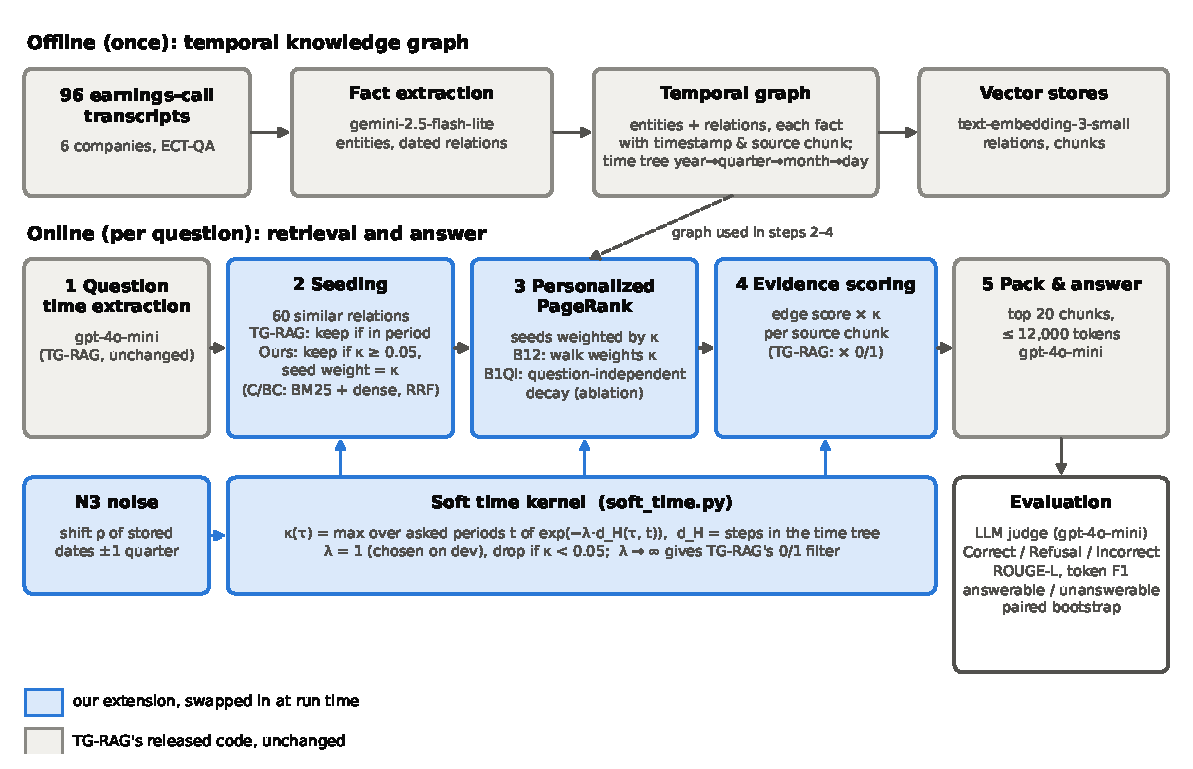
\includegraphics[width=\textwidth]{figures/architecture.pdf}
  \caption{System architecture. Grey: the base system's released code, unchanged. Blue: our extension, swapped in at run time. The soft kernel feeds seeding, the walk and evidence scoring; noise injection changes stored timestamps before the kernel reads them.}
  \label{fig:arch}
\end{figure}

\section{Method}
\subsection{Setting and baseline}
The graph $G = (V, E)$ has entity nodes; an edge can hold several facts $f = (u_f, v_f, \tau_f, c_f)$ with two entities, a timestamp and the source chunk $c_f$. Timestamps take one of four forms (YYYY, YYYY-QN, YYYY-MM, YYYY-MM-DD) and form a tree in which quarters lie below years, months below quarters and days below months; $p(\tau)$ is the path of $\tau$ from the root. A question $q$ names periods $T_q$, read by the answering model. Retrieval selects chunks $C_q$ under a token budget $B$:
\begin{equation}
  C_q = \operatorname{top\text{-}}k_{\,c}\; S(c) \quad \text{s.t.} \quad \textstyle\sum_{c \in C_q} |c| \le B,
  \label{eq:select}
\end{equation}
with $k = 20$ and $B = 12{,}000$ tokens. TG-RAG's decision for a fact is the 0/1 filter
\begin{equation}
  h(\tau) = \mathbf{1}\!\left[\tau \in \operatorname{desc}(T_q)\right],
  \label{eq:hard}
\end{equation}
where $\operatorname{desc}(T_q)$ contains the asked periods and their sub-periods. Its retrieval (i) takes the $3k = 60$ relations most similar to $q$, (ii) keeps those with $h = 1$ as seeds, (iii) runs PPR from the seed entities with damping 0.85 and keeps the top $2k = 40$ entities, (iv) scores chunks from facts on edges between kept entities, and (v) packs the best chunks into the budget.

\subsection{Soft temporal kernel (N1)}
The tree distance between a stored timestamp $\tau$ and an asked period $t$ is
\begin{equation}
  d_H(\tau, t) =
  \begin{cases}
    0, & \tau \text{ is or lies inside } t,\\
    |p(\tau)| + |p(t)| - 2\ell, & \text{otherwise,}
  \end{cases}
  \label{eq:dist}
\end{equation}
where $\ell = |\operatorname{lcp}(p(\tau), p(t))|$ is the length of the longest common prefix of the two paths, and different years meet at a virtual root. Thus 2023-Q1 and 2023-Q2 are 2 apart, 2022-Q4 and 2023-Q1 are 4 apart, and a year-level fact is 1 from a quarter of the same year. The kernel is
\begin{equation}
  \kappa(\tau) = \max_{t \in T_q} \exp\big(-\lambda\, d_H(\tau, t)\big),
  \label{eq:kappa}
\end{equation}
and a fact is kept only if $\kappa(\tau_f) \ge \kappa_{\min} = 0.05$. Unparseable timestamps get $\kappa = 0$, and questions without periods give every fact weight 1, both as in TG-RAG. Since $\exp(-\lambda d) \to \mathbf{1}[d = 0]$,
\begin{equation}
  \lim_{\lambda \to \infty} \kappa(\tau) = h(\tau),
  \label{eq:limit}
\end{equation}
so TG-RAG is a special case. With $\lambda = 1$, facts at distance 0, 1, 2 get 1, 0.368 and 0.135; distance 3 gives $e^{-3} = 0.0498 < \kappa_{\min}$ and is dropped.

\subsection{Kernel throughout retrieval (N2)}
\textbf{Seeding.} A seed entity's weight is the largest kernel value among the kept candidate facts $R_q$ that touch it,
\begin{equation}
  w(v) = \max_{f \in R_q:\; v \in f,\; \kappa(\tau_f) \ge \kappa_{\min}} \kappa(\tau_f).
  \label{eq:seed}
\end{equation}
\textbf{Walk.} PPR restarts in proportion to the seed weights (TG-RAG restarts uniformly):
\begin{equation}
  \bm{\pi} = \alpha P^{\top} \bm{\pi} + (1 - \alpha)\, \mathbf{p}, \quad p(v) = \frac{w(v)}{\sum_u w(u)}, \quad \alpha = 0.85,
  \label{eq:ppr}
\end{equation}
with $P_{uv} \propto \omega(u, v)$. Variant B1 keeps $\omega = 1$. Variant B12 sets $\omega(u, v) = \max_{f \text{ on } (u,v)} \kappa(\tau_f)$, zeroed below $\kappa_{\min}$, with untimed edges at 1.

\textbf{Scoring.} For edges between the top entities, each kept fact adds its weight times the endpoint scores to its chunk:
\begin{equation}
  S(c) = \prod_{\gamma \in \Gamma_c} (1 + \gamma) \sum_{f:\, c_f = c} \kappa(\tau_f)\,\big[\pi(u_f) + \pi(v_f)\big],
  \label{eq:score}
\end{equation}
where $\Gamma_c$ are the similarities of seed relations on the contributing edges. Under the hard filter, $\kappa$ in (\ref{eq:score}) is $h$.

\textbf{Question-independent ablation (B1QI).} Following the idea of time-decayed links \cite{sun2025dygrag}, a fact's coherence with the facts $N(f)$ sharing one of its entities is
\begin{equation}
  \operatorname{coh}(f) = \frac{1}{|N(f)|} \sum_{f' \in N(f)} e^{-\alpha d_H(\tau_f, \tau_{f'})},
  \label{eq:coh}
\end{equation}
with $\alpha = 1$, and the walk weight of an edge is the largest coherence of its facts, $\omega(u, v) = \max_{f \text{ on } (u,v)} \operatorname{coh}(f)$. B1QI equals B12 except for these walk weights, which ignore the question.

\subsection{Hybrid seeding (S1) and noise protocol (N3)}
In variants C (hard filter) and BC (B12), candidates are chosen per asked period: the relations admitted for that period are ranked by dense similarity and by BM25 and fused by
\begin{equation}
  \operatorname{RRF}(r) = \sum_{i} \frac{1}{k + \operatorname{rank}_i(r)}, \qquad k = 60,
  \label{eq:rrf}
\end{equation}
where $i$ runs over the dense and the BM25 ranking, each period contributing $\lceil 60/|T_q| \rceil$ candidates. For robustness, a share $\rho \in \{0.1, 0.2, 0.3\}$ of stored timestamps is moved by one quarter (one year for year-level stamps). The decision and the direction come from a SHA-256 hash of (seed 13, entity pair, timestamp), so the same fact is corrupted identically for every method and the comparison stays paired.

\subsection{Implementation}
The base system's code is left untouched; our package replaces its retrieval function at run time, so all methods share the graph, question parser, answer prompt and models (Fig.~\ref{fig:arch}). The retriever records every candidate fact with its timestamp, weight and decision. Twenty-four unit tests check the distances, the kernel limit, noise determinism, the question-independence of B1QI, and that the re-implemented baseline returns exactly the base function's chunks on a synthetic graph.


\begin{figure}[t]
  \centering
  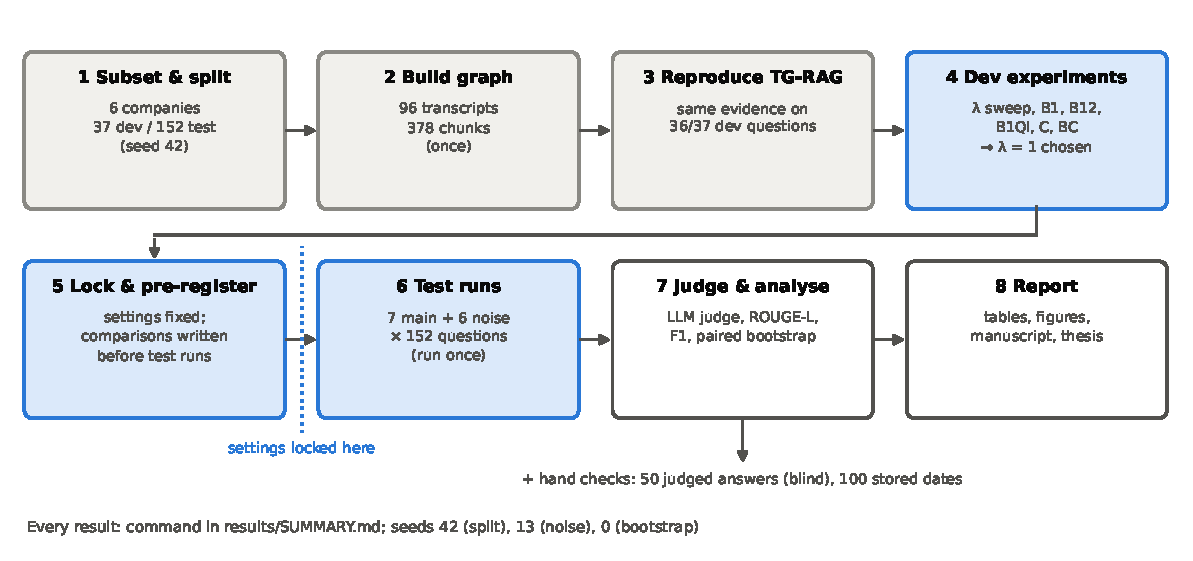
\includegraphics[width=0.9\textwidth]{figures/workflow.pdf}
  \caption{Workflow. Settings were locked on the development set before the test set was run once.}
  \label{fig:workflow}
\end{figure}

\section{Experimental Setup}
\textbf{Data.} We use all transcripts of six ECT-QA companies for 2020--2023 (Crocs, EOG Resources, Home Depot, JD.com, Skechers, Yum China): 96 transcripts and 189 questions, split once into 37 development and 152 test questions, stratified by type (seed 42). The test set has 116 answerable and 36 unanswerable questions (32 about periods outside the corpus, 4 about unreported facts). By type it has 62 multi-time, 37 single-time multi-keyword, 33 single-time multi-company and 20 relative-time questions. The subset keeps the model-call budget within USD 10--30.

\textbf{Graph and models.} One graph, shared by all methods, was built with the base pipeline using gemini-2.5-flash-lite: 96 documents, 378 chunks and 8,476 relation records (8,408 dated facts with a description). Embeddings use text-embedding-3-small; reading the question's periods, answering and judging use gpt-4o-mini at temperature 0 with the response cache. All models were reached through one OpenRouter endpoint on a laptop without a GPU.

\textbf{Methods.} The reproduced TG-RAG baseline; the released TG-RAG code (development only, as a check); naive RAG over the same chunks; and the variants B1, B12, B1QI, C and BC (Section~III). All use $k = 20$, 60 candidates and a 12,000-token context.

\textbf{Protocol.} $\lambda$ was chosen on the development set from $\{0.25, 0.5, 1, 2, 4, 1000\}$ by a rule fixed beforehand: take the highest overall Correct, and within 0.03 prefer the larger $\lambda$ or the simpler variant. This gave B1 with $\lambda = 1$. The test comparisons were then pre-registered: the main claim is B1 against the baseline overall and on answerable questions; the secondary comparisons are B12 against B1QI, B12 against B1, and C against the baseline; robustness is B1 against the baseline at each noise rate. Every test configuration was run once (Fig.~\ref{fig:workflow}).

\textbf{Metrics.} A judge lists the factual elements of the gold answer and labels each element in the prediction as correct, refused or incorrect, giving
\begin{equation}
  \operatorname{Correct}(q) = \frac{n_{\text{correct}}}{n_{\text{correct}} + n_{\text{refusal}} + n_{\text{incorrect}}}
  \label{eq:correct}
\end{equation}
for answerable questions, and $n_{\text{refused}}/(n_{\text{refused}} + n_{\text{incorrect}})$ for unanswerable ones. The released code has no evaluation script, so the prompts are our own wording of the published protocol. Correct is also reported separately for answerable and unanswerable questions. ROUGE-L and token F1 ($2PR/(P+R)$) are computed on answerable questions. Differences use a paired bootstrap over questions,
\begin{equation}
  \Delta = \frac{1}{n} \sum_q \big(S_{\text{ours}}(q) - S_{\text{base}}(q)\big),
  \label{eq:delta}
\end{equation}
with 1,000 resamples (seed 0), the 2.5th/97.5th percentile interval and the one-sided $p = \Pr(\Delta^* \le 0)$. A gain is significant when the interval lies above zero.


\begin{figure}[t]
  \centering
  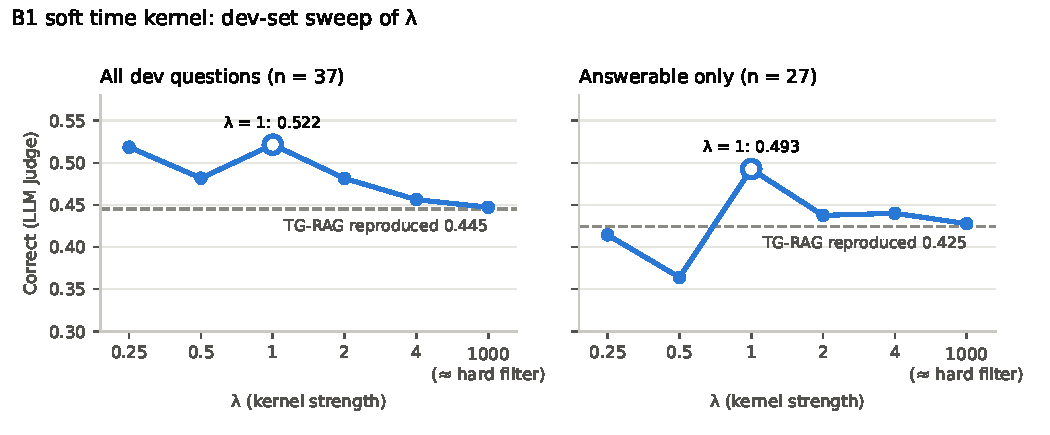
\includegraphics[width=0.9\textwidth]{figures/lambda_sweep_dev.pdf}
  \caption{Development set: Correct of B1 for each $\lambda$, all questions and answerable only; dashed line = reproduced baseline.}
  \label{fig:sweep}
\end{figure}

\section{Results}
\subsection{Baseline verification and development set}
Our re-implemented baseline selects the same chunks as the released code on 36 of 37 development questions; the exception is an unanswerable question with one extra chunk. B1 with $\lambda = 1000$ scores 0.447 against 0.445 for the baseline, with 95\% of questions receiving identical evidence, which confirms (\ref{eq:limit}) in practice. On the development set B1 ($\lambda = 1$) reached 0.522 against 0.445 ($+0.077$, 95\% CI $[-0.050, 0.208]$, $p = 0.113$; Fig.~\ref{fig:sweep}). On three answerable questions the hard filter found no seed at all, while B1 found 11, 11 and 7 seeds. With 37 questions, nothing on the development set was significant.

\subsection{Test set}
Table~\ref{tab:main} gives the test results. \textbf{The pre-registered main claim is not supported}: B1 scores 0.603 against 0.599 ($+0.004$, $[-0.049, +0.059]$, $p = 0.445$), and 0.554 against 0.540 on answerable questions ($+0.014$, $[-0.049, +0.083]$, $p = 0.334$). ROUGE-L and F1 change by less than 0.01. Naive RAG leads on unanswerable questions (0.944) because it refuses often, but it is significantly worse on answerable ones ($-0.114$, $[-0.211, -0.022]$). Our baseline's 0.599 coincides with the score TG-RAG reports on the full benchmark; since the subset, judge prompts and models differ, the two are not comparable.

\begin{table*}[t]
\centering
\caption{Test set (152 questions). Correct from the judge; ROUGE-L and F1 on answerable questions; $\Delta$: paired bootstrap against the reproduced baseline.}
\label{tab:main}
\resizebox{\textwidth}{!}{%
\begin{tabular}{lccccccc}
\toprule
Method & All & Ans. (116) & Unans. (36) & ROUGE-L & F1 & $\Delta$ all [95\% CI] & $\Delta$ ans. [95\% CI] \\
\midrule
TG-RAG, reproduced & 0.599 & 0.540 & 0.792 & 0.185 & 0.218 & -- & -- \\
Naive RAG & 0.548 & 0.426 & 0.944 & 0.195 & 0.228 & $-0.051$ [$-0.126$, $+0.025$] & $-0.114$ [$-0.211$, $-0.022$] \\
\textbf{B1, soft kernel ($\lambda = 1$)} & \textbf{0.603} & \textbf{0.554} & 0.764 & 0.190 & 0.224 & $+0.004$ [$-0.049$, $+0.059$] & $+0.014$ [$-0.049$, $+0.083$] \\
B12, kernel also in walk & 0.605 & 0.555 & 0.764 & 0.193 & 0.226 & $+0.005$ [$-0.050$, $+0.069$] & $+0.016$ [$-0.051$, $+0.091$] \\
B1QI, question-independent walk & 0.605 & 0.547 & 0.792 & 0.193 & 0.225 & $+0.006$ [$-0.049$, $+0.064$] & $+0.007$ [$-0.059$, $+0.085$] \\
C, hybrid seeding, hard filter & 0.561 & 0.468 & 0.861 & 0.179 & 0.210 & $-0.038$ [$-0.094$, $+0.020$] & $-0.071$ [$-0.136$, $-0.003$] \\
BC, B12 + hybrid seeding & 0.626 & 0.522 & 0.958 & 0.189 & 0.219 & $+0.026$ [$-0.039$, $+0.094$] & $-0.017$ [$-0.084$, $+0.055$] \\
\bottomrule
\end{tabular}}
\end{table*}

\subsection{Ablations}
The three kernel variants lie within 0.002 of each other. Question-aware decay is no better than question-independent decay (B12 vs B1QI: $-0.000$, $[-0.036, +0.039]$), and the kernel in the walk adds nothing (B12 vs B1: $+0.001$, $[-0.037, +0.044]$). Hybrid seeding with the hard filter (C) is the only significant difference, and it is negative on answerable questions ($-0.071$). BC has the highest overall score, 0.626, but its gain comes from unanswerable questions (0.958); on answerable questions it is below the baseline. Selecting it now would mean choosing on the test set.

\subsection{Robustness}
As the share of shifted timestamps grows, the baseline stays at 0.600 at 10\% and falls to 0.575 and 0.566, while B1 does not fall (0.582, 0.606, 0.627; Table~\ref{tab:robust}, Fig.~\ref{fig:robust}). At 30\% the gap is $+0.061$ $[+0.005, +0.120]$, $p = 0.019$. This is one of six robustness tests, and with a Bonferroni correction ($p < 0.025/6 \approx 0.004$) none passes. B1 also scored higher with 30\% noise than without noise, which shows that run-to-run variation is of the same size as the effect. We therefore read this as a trend consistent with N3.

\begin{table}[t]
\centering
\caption{Robustness (test set, Correct). $\Delta$ = B1 minus baseline.}
\label{tab:robust}
\setlength{\tabcolsep}{3.5pt}
\begin{tabular}{lccc}
\toprule
Shifted & Baseline & B1 & $\Delta$ all [95\% CI], $p$ \\
\midrule
0\% & 0.599 & 0.603 & $+0.004$ [$-0.049$, $+0.059$], 0.445 \\
10\% & 0.600 & 0.582 & $-0.018$ [$-0.081$, $+0.043$], 0.719 \\
20\% & 0.575 & 0.606 & $+0.031$ [$-0.027$, $+0.096$], 0.155 \\
30\% & 0.566 & 0.627 & $+0.061$ [$+0.005$, $+0.120$], 0.019 \\
\bottomrule
\end{tabular}
\end{table}

\begin{figure}[t]
  \centering
  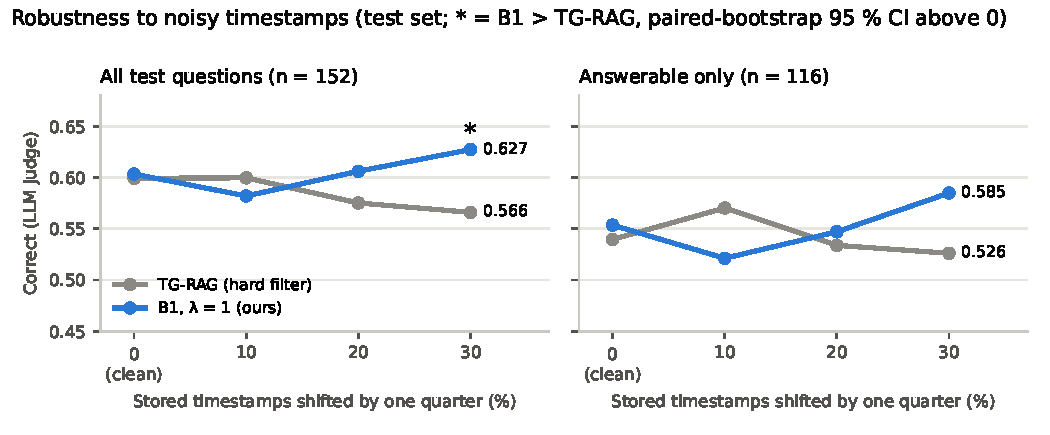
\includegraphics[width=\columnwidth]{figures/robustness_test.pdf}
  \caption{Correct versus the share of stored timestamps shifted by one quarter (test set). A star marks an interval of the difference lying above zero.}
  \label{fig:robust}
\end{figure}

\subsection{Where the methods differ (exploratory)}
On the 116 answerable test questions, B1 changes the retrieved context on 110. It is better than the baseline on 35, worse on 28 and tied on 53; the gains ($+12.90$) and losses ($-11.27$) nearly cancel. By type (Fig.~\ref{fig:types}), B1 helps on multi-time questions (0.522 to 0.596) and single-time multi-keyword questions (0.647 to 0.732). It hurts on single-time multi-company questions (0.697 to 0.516; worse on 13 of 22 answerable ones) and on relative-time questions (0.590 to 0.533). A plausible, untested explanation is that neighbouring-quarter facts help to fill multi-period questions but compete for the fixed context with exact-period facts about the other companies. Questions with no seed under the hard filter occurred on only 2 of 116 answerable test questions (3 of 27 on development); B1 scored 0.458 against 0.000 on them.

\begin{figure}[t]
  \centering
  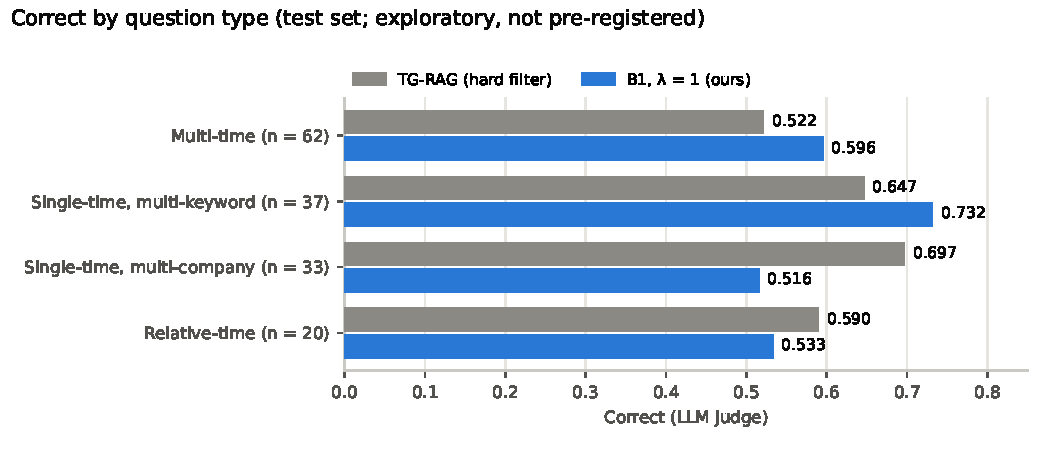
\includegraphics[width=\columnwidth]{figures/per_type_test.pdf}
  \caption{Correct by question type, baseline vs B1 (test set, exploratory).}
  \label{fig:types}
\end{figure}

\section{Additional Technical Detail}
\subsection{Retrieval algorithm}
Algorithm~\ref{alg:retrieve} gives the full retrieval of variant B1; B12 and B1QI differ only in the edge weights used by the walk (line 7).

\begin{algorithm}[t]
\caption{Soft-kernel retrieval (variant B1) for one question}
\label{alg:retrieve}
\begin{algorithmic}[1]
\Require question $q$, periods $T_q$, graph $G$, $\lambda{=}1$, $\kappa_{\min}{=}0.05$, $k{=}20$, $B{=}12{,}000$
\State $R_q \gets$ the $3k$ relations most similar to $q$
\ForAll{$f \in R_q$} \Comment{seeding, (\ref{eq:kappa}), (\ref{eq:seed})}
  \State $\kappa_f \gets \max_{t \in T_q} \exp(-\lambda\, d_H(\tau_f, t))$; skip $f$ if $\kappa_f < \kappa_{\min}$
  \State $w(u_f) \gets \max(w(u_f), \kappa_f)$; \; $w(v_f) \gets \max(w(v_f), \kappa_f)$
\EndFor
\If{no seed} \Return $\emptyset$ \EndIf
\State $\bm{\pi} \gets$ PPR with restart $\propto w$, damping 0.85, weights $\omega$ \Comment{(\ref{eq:ppr})}
\State $U \gets$ top-$2k$ entities by $\pi$
\ForAll{edges $(u,v)$, $u, v \in U$, facts $f$ on them with $\kappa(\tau_f) \ge \kappa_{\min}$}
  \State $S(c_f) \gets S(c_f) + \kappa(\tau_f)[\pi(u) + \pi(v)]$ \Comment{(\ref{eq:score})}
\EndFor
\State $S(c) \gets S(c) \cdot \prod_{\gamma \in \Gamma_c}(1 + \gamma)$ for every chunk
\State \Return top-$k$ chunks by $S$, packed greedily within $B$
\end{algorithmic}
\end{algorithm}

\subsection{Kernel weights}
Table~\ref{tab:weights} lists the weights for the locked setting. Facts up to two tree steps away are kept; the boundary case $e^{-3} = 0.0498$ falls just under $\kappa_{\min}$.

\begin{table}[t]
\centering
\caption{Kernel weights for $\lambda = 1$, $\kappa_{\min} = 0.05$}
\label{tab:weights}
\begin{tabular}{lccc}
\toprule
Stored timestamp vs asked period & $d_H$ & $\kappa$ & Used \\
\midrule
inside the asked period & 0 & 1.000 & yes \\
year fact, quarter of the same year asked & 1 & 0.368 & yes \\
neighbouring quarter, same year & 2 & 0.135 & yes \\
year fact, quarter of another year asked & 3 & 0.050 & no \\
neighbouring quarter across a year boundary & 4 & 0.018 & no \\
timestamp not in a valid form & -- & 0 & no \\
\bottomrule
\end{tabular}
\end{table}

\ifextended
\subsection{Noise protocol in detail}
For a fact on entity pair $(u, v)$ with timestamp $\tau$, the first eight bytes of $\operatorname{SHA256}(13 \,\|\, \operatorname{sort}(u, v) \,\|\, \tau)$, read as an integer and divided by $2^{64}$, give $h \in [0, 1)$. If $h < \rho$ the timestamp is moved by one quarter, earlier or later according to the parity of the ninth byte; year-level timestamps move by one year, and month and day timestamps by three months. Because $h$ depends only on the fact, the corrupted graph is identical for every method and every run.

\subsection{Implementation and tests}
The extension consists of four modules: tree distance, kernel and noise (\texttt{soft\_time.py}); the retrieval variants and the run-time swap (\texttt{retriever.py}); model-name mapping for a single provider key (\texttt{openrouter.py}); and a chunk index for naive RAG (\texttt{naive\_index.py}). The scripts answer questions resumably, judge and analyse runs, and rebuild every table and figure from the saved files. The 24 unit tests cover tree paths and distances (5 tests in the soft-time module), the retriever (11 tests, including identity with the base function on a synthetic graph and the $\lambda = 1000$ limit), model mapping (2), the naive index (1), and the hand-check tools (5).

\fi
\section{Additional Results}
\subsection{Development set}
Table~\ref{tab:dev} gives all development runs. The released code scored slightly below our reproduction (0.418 vs 0.445) although the two retrieve the same evidence on 36 of 37 questions; we did not trace the cause of this small difference, and all comparisons use our reproduction, which runs in exactly the same pipeline as the variants. On the three questions where the hard filter found no seed (base-6, base-542, base-519), B1 scored 0.33, 1.00 and 0.40.

\begin{table}[t]
\centering
\caption{Development set (37 questions: 27 answerable, 10 unanswerable), Correct}
\label{tab:dev}
\begin{tabular}{lccc}
\toprule
Run & All & Ans. & Unans. \\
\midrule
TG-RAG, reproduced & 0.445 & 0.425 & 0.500 \\
TG-RAG, released code & 0.418 & 0.388 & 0.500 \\
Naive RAG & 0.488 & 0.336 & 0.900 \\
\textbf{B1, $\lambda = 1$} & \textbf{0.522} & \textbf{0.493} & 0.600 \\
B12 & 0.523 & 0.494 & 0.600 \\
B1QI & 0.506 & 0.434 & 0.700 \\
C & 0.497 & 0.422 & 0.700 \\
BC & 0.511 & 0.404 & 0.800 \\
\midrule
\multicolumn{4}{l}{$\lambda$ sweep (B1, all questions): 0.25: 0.519, 0.5: 0.482,} \\
\multicolumn{4}{l}{1: 0.522, 2: 0.481, 4: 0.456, 1000: 0.447} \\
\bottomrule
\end{tabular}
\end{table}

\subsection{Secondary comparisons and robustness on answerable questions}
Table~\ref{tab:pairs} reports the two pre-registered pairs that do not involve the baseline, and the robustness comparison restricted to answerable questions.

\begin{table}[t]
\centering
\caption{Secondary comparisons (test set)}
\label{tab:pairs}
\resizebox{\linewidth}{!}{%
\begin{tabular}{lcc}
\toprule
Comparison & $\Delta$ all [95\% CI], $p$ & $\Delta$ ans. [95\% CI], $p$ \\
\midrule
B12 vs B1QI & $-0.000$ [$-0.036$, $+0.039$], 0.461 & $+0.008$ [$-0.043$, $+0.058$], 0.368 \\
B12 vs B1 & $+0.001$ [$-0.037$, $+0.044$], 0.435 & $+0.002$ [$-0.045$, $+0.054$], 0.462 \\
B1 vs base, 10\% noise & $-0.018$ [$-0.081$, $+0.043$], 0.719 & $-0.049$ [$-0.123$, $+0.025$], 0.904 \\
B1 vs base, 20\% noise & $+0.031$ [$-0.027$, $+0.096$], 0.155 & $+0.013$ [$-0.059$, $+0.092$], 0.351 \\
B1 vs base, 30\% noise & $+0.061$ [$+0.005$, $+0.120$], 0.019 & $+0.059$ [$-0.004$, $+0.126$], 0.036 \\
\bottomrule
\end{tabular}}
\end{table}

\subsection{Per-question breakdown}
Table~\ref{tab:types} splits the per-question comparison on answerable test questions by type.

\begin{table}[t]
\centering
\caption{B1 vs baseline per answerable test question, by type (exploratory)}
\label{tab:types}
\begin{tabular}{lccccc}
\toprule
Question type & $n$ & Better & Worse & Tied & Net \\
\midrule
Multi-time & 50 & 18 & 7 & 25 & $+4.58$ \\
Single-time, multi-keyword & 30 & 12 & 6 & 12 & $+2.15$ \\
Single-time, multi-company & 22 & 3 & 13 & 6 & $-4.97$ \\
Relative-time & 14 & 2 & 2 & 10 & $-0.13$ \\
\midrule
All answerable & 116 & 35 & 28 & 53 & $+1.63$ \\
\bottomrule
\end{tabular}
\end{table}

\ifextended
\subsection{Reasoning types}
Fig.~\ref{fig:reasoning} splits the test set by what the question asks the model to do. B1 is slightly ahead on comparison questions (0.403 against 0.379, $n = 46$) and on lists of values (0.652 against 0.645, $n = 70$), and identical on questions about periods outside the corpus (0.781, $n = 32$). The largest gap, on unanswerable questions about unreported facts (0.625 against 0.875), rests on only four questions, where one answer moves the score by 0.25; we do not read anything into it.

\begin{figure}[t]
  \centering
  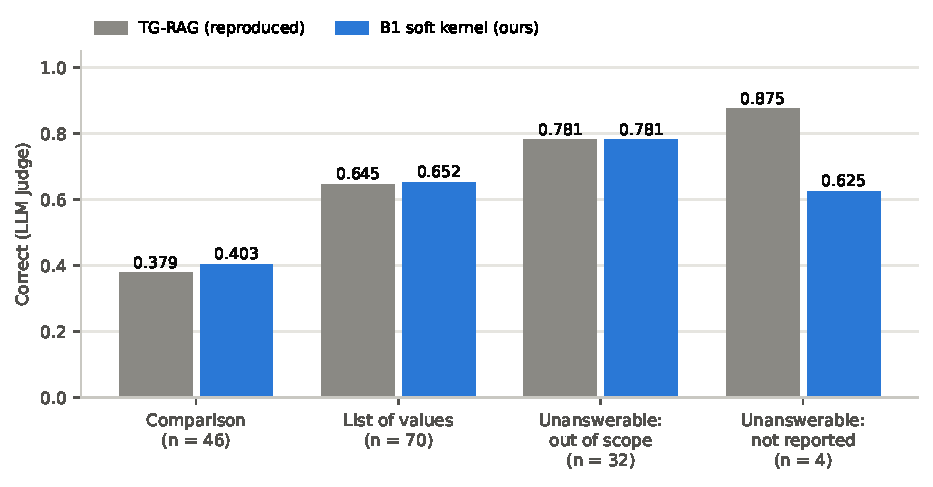
\includegraphics[width=0.85\textwidth]{figures/reasoning_type_test.pdf}
  \caption{Correct by reasoning type, baseline vs B1 (test set, exploratory).}
  \label{fig:reasoning}
\end{figure}

\subsection{Context size and running time}
Fig.~\ref{fig:efficiency} reports the mean number of context tokens sent to the answering model and the mean wall-clock time per question. All graph variants use between 11,039 and 11,462 tokens of the 12,000-token budget, so the variants differ in which facts they send, not in how much text. The timing panel is not a fair speed comparison: the baseline ran first, before the model-call cache was warm (5.94 s per question against 3.13--3.97 s for the later runs), and no separate latency benchmark was made. We therefore make no claim about speed.

\begin{figure}[t]
  \centering
  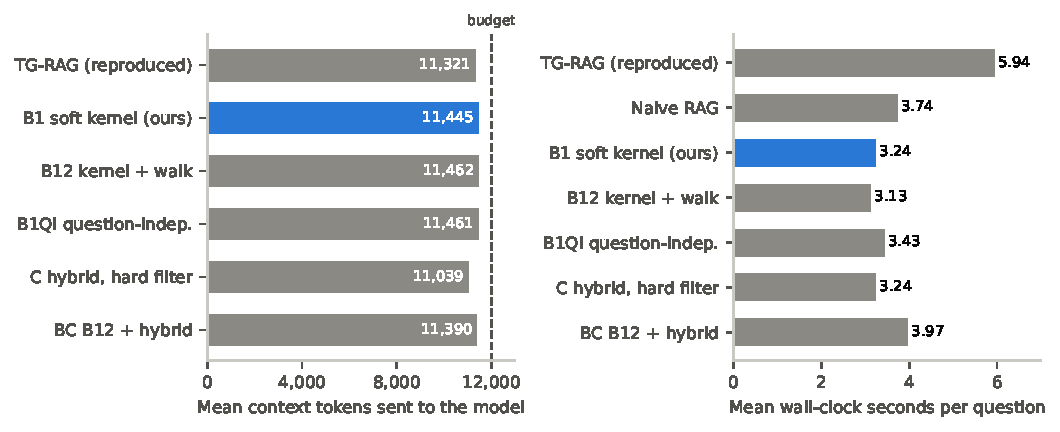
\includegraphics[width=0.95\textwidth]{figures/efficiency_test.pdf}
  \caption{Mean context tokens (left; naive RAG does not record this) and mean wall-clock seconds per question (right) on the test set. Timing differences mainly reflect the response cache, since the baseline ran first.}
  \label{fig:efficiency}
\end{figure}
\fi

\subsection{Case study}
For development question base-6 (EOG Resources' free cash flow in 2021-Q4, 2022-Q1 and 2022-Q2; gold: \$2 billion, \$2.3 billion, nearly \$1.3 billion), the question parser read only 2021-Q4. No candidate carried exactly that quarter, so the baseline kept 0 of 60 candidates and its answer contained three invented figures (judge score 0.00). B1 kept 13 candidates, mostly from 2021-Q1 to Q3 at weight 0.135, sent 11 chunks and answered 2021-Q4 correctly while stating the other quarters were unavailable (0.33). Facts from 2022-Q1 (weight 0.018) and from full years 2020 and 2023 (0.050) were dropped. The missing quarters are a limitation of the shared parser, which we keep unchanged for fairness.

\ifextended
\section{Threats to Validity and Deviations}
\textbf{Internal validity.} The baseline is verified against the released code, every method shares the same graph, parser, prompts and models, and answers are deterministic. The remaining internal threat is the judge: one model with our own prompts. Its agreement with a human reader on 50 blind answers has not yet been measured.

\textbf{External validity.} One benchmark, six companies, one graph and one language-model family; results may differ for other sectors, other graph builders or larger models.

\textbf{Statistical conclusion validity.} The test set gives intervals of about $\pm 0.05$, the robustness result does not survive a multiple-testing correction, and a single noise seed was used.

\textbf{Deviations from the original plan.} The first plan measured robustness on the combined variant BC; the registered comparison uses B1, the variant selected on the development set. A sweep of the B1QI decay rate was planned, but only $\alpha = 1$ was run. A fiscal-year alias for timestamps is implemented but was not enabled. None of these choices was made after seeing test results.

\fi


\section{Discussion and Limitations}
Softening the date filter does not raise average accuracy on held-out questions. The kernel works as intended: it recovers evidence when the filter finds none and it helps multi-period questions. But it also lets nearby facts crowd out exact ones in single-period, multi-entity questions, and the two effects cancel. The development gain of $+0.077$ vanished on test. The 37-question interval was very wide, and zero-evidence cases were rarer on test. Fixing the settings and the comparisons in advance is what makes this null result trustworthy rather than a tuning artefact. The robustness result is the most encouraging finding, but it rests on one significant test out of six and is within run-to-run variation.

\textbf{Limitations.} (i) With 152 test questions, intervals of about $\pm 0.05$ cannot detect smaller effects. (ii) A single judge model with our own prompt wording produces the main metric. A blind check of 50 judged answers against a human reader is prepared but not yet scored. ROUGE-L and F1 are low for every system ($\approx 0.19$) because gold answers are short. (iii) Each configuration was run once, and the noise test used one noise seed. (iv) One-quarter shifts model only one kind of error; malformed timestamps (9.9\%) get weight 0 under both methods. (v) Six of 24 companies; absolute scores are not comparable with published full-benchmark numbers.

\section{Conclusion}
We replaced the hard temporal filter of a temporal graph RAG system with a soft kernel over a calendar tree. The kernel is a strict generalisation with one parameter, and we evaluated it under a pre-registered protocol on earnings-call QA. It did not improve average accuracy, and question-aware decay was no better than question-independent decay. Its benefit appeared mainly when stored timestamps were noisy, and even there the evidence is a trend. Promising next steps, each needing a new development and test cycle, are a kernel strength per question type, reserving context for exact-period facts, normalising malformed timestamps, and repeating the noise study with several seeds. Code, settings and the command behind every number are released with this paper.


\bibliographystyle{IEEEtranN}
\bibliography{references}
\end{document}
